\section{Installation of Spark}
\label{c:spark-local-installation}
\FILENAME\

In this section we will discuss how to install Spark 2.3.0 in Ubuntu 16.04.

\subsection{Prerequisits}

We assume that you have ssh, and rsync installed and
use emacs as editor. 

\begin{lstlisting}
sudo apt-get install ssh
sudo apt-get install rsync
sudo apt-get install emacs
\end{lstlisting}

\subsection{Installation of Java}

First download Java 8.

\begin{lstlisting}
mkdir -p ~/cloudmesh/bin
cd ~/cloudmesh/bin
wget -c --header "Cookie: oraclelicense=accept-securebackup-cookie" "http://download.oracle.com/otn-pub/java/jdk/8u161-b12/2f38c3b165be4555a1fa6e98c45e0808/jdk-8u161-linux-x64.tar.gz"
tar xvzf jdk-8u161-linux-x64.tar.gz
\end{lstlisting}

Then add the environmental variables to the bashrc file. 

\begin{lstlisting}
emacs ~/.bashrc
\end{lstlisting}

\begin{lstlisting}
export JAVA_HOME=~/cloudmesh/bin/jdk1.8.0_161
export PATH=$JAVA_HOME/bin:$PATH
\end{lstlisting}

Source the bashrc file after adding the environmental variables.

\begin{lstlisting}
  source ~/.bashrc
\end{lstlisting}

\subsection{Install Spark with Hadoop}\label{s:s:install-spark-with-hadoop}

\begin{NOTE}
  Here we use Spark packaged with Hadoop. In this package Spark uses
  Hadoop 2.7.0 in the packaged version. Note that in
  Section~\ref{s:hadoop-local-installation} we use for the vanilla
  Hadoop instalation Hadoop 3.0.0.
\end{NOTE}

Create the base directories and go to the directory.

\begin{lstlisting}
mkdir -p ~/cloudmesh/bin
cd ~/cloudmesh/bin
\end{lstlisting}
  
Then download Spark 2.3.0 as follows. 

\begin{lstlisting}
wget https://www.apache.org/dyn/closer.lua/spark/spark-2.3.0/spark-2.3.0-bin-hadoop2.7.tgz
\end{lstlisting}

Now extract the file,

\begin{lstlisting}
tar xzf spark-2.3.0-bin-hadoop2.7.tgz
mv spark-2.3.0-bin-hadoop2.7 spark-2.3.0
\end{lstlisting}

\subsection{Spark Environment Variables}

Open up bashrc file and add environmental variables as follows.

\begin{lstlisting}
emacs ~/.bashrc  
\end{lstlisting}

Go to the last line and add the following content.

\begin{lstlisting}
export SPARK_HOME=~/cloudmesh/bin/spark-2.3.0
export PATH=$SPARK_HOME/bin:$PATH
\end{lstlisting}  

Source the bashrc file.

\begin{lstlisting}
source ~/.bashrc
\end{lstlisting}

\subsection{Test Spark Installation}

Open up a new terminal and then run the following command.

\begin{lstlisting}
spark-shell
\end{lstlisting}

If it has been configured properly, it will display the following content.

\begin{lstlisting}
Spark context Web UI available at http://192.168.1.66:4041
Spark context available as 'sc' (master = local[*], app id = local-1521674331361).
Spark session available as 'spark'.
Welcome to
      ____              __
     / __/__  ___ _____/ /__
    _\ \/ _ \/ _ `/ __/  '_/
   /___/ .__/\_,_/_/ /_/\_\   version 2.3.0
      /_/
         
Using Scala version 2.11.8 (Java HotSpot(TM) 64-Bit Server VM, Java 1.8.0_151)
Type in expressions to have them evaluated.
Type :help for more information.
\end{lstlisting}

\begin{NOTE}
  Please check the console LOGS and find the port number on which the
  Spark Web UI is hosted. It will show something like:

  Spark context Web UI available at: <some url>
\end{NOTE}

Then take a look the following address in the browser.
\begin{lstlisting}
http://localhost:4041
\end{lstlisting}

If you see the Spark Dashboard, then you can realize you have installed Spark
successfully.

\subsection{Install Spark With Custom Hadoop}

Installing Spark with pre-existing Hadoop version is favorable, if you
want to use the latest features from the latest Hadoop version or when
you need a specific Hadoop version depending on the external
dependencies to your project.

First we need to download the Spark packaged without Hadoop.

\begin{lstlisting}
  mkdir -p ~/cloudmesh/bin
  cd ~/cloudmesh/bin
\end{lstlisting}
  
Then download Spark 2.3.0 as follows. 

\begin{lstlisting}
wget http://mirrors.ibiblio.org/apache/spark/spark-2.3.0/spark-2.3.0-bin-without-hadoop.tgz
\end{lstlisting}

Now extract the file,

\begin{lstlisting}
  tar xzf spark-2.3.0-bin-without-hadoop.tgz  
\end{lstlisting}

Then add the environmental variables,

\begin{NOTE}
  If you have already installed Spark with Hadoop by following section
  \ref{s:s:install-spark-with-hadoop} please update the current SPARK
  HOME variable with the new path.
\end{NOTE}

\begin{lstlisting}
  emacs ~/.bashrc  
\end{lstlisting}

Go to the last line and add the following content.

\begin{lstlisting}
export SPARK_HOME=~/cloudmesh/bin/spark-2.3.0-bin-without-hadoop
export PATH=$SPARK_HOME/bin:$PATH
\end{lstlisting}  

Source the bashrc file.

\begin{lstlisting}
source ~/.bashrc
\end{lstlisting}

\subsection{Configuring Hadoop}

Now we must add the current Hadoop version that we are using for
Spark. Open up a new terminal and then run the following.

\begin{lstlisting}
cd $SPARK_HOME
\end{lstlisting}

\begin{lstlisting}
  cd conf
  cp spark-env.sh.template spark-evn.sh
\end{lstlisting}

Now we need to add a new line to show the current path to
hadoop installation. Add the following variable in to the
spark-env.sh file.

\begin{lstlisting}
  emacs spark-env.sh
  export SPARK_DIST_CLASSPATH=$($HADOOP_HOME/bin/hadoop classpath)
\end{lstlisting}

\begin{figure}
\centering
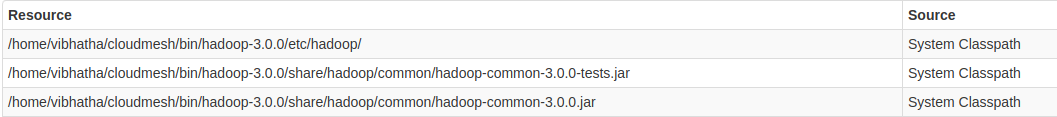
\includegraphics[width=\textwidth,height=\textheight,keepaspectratio]{images/spark-hadoop.png}
\caption{Spark Web UI - Hadoop Path}
\end{figure}


\subsection{Test Spark Installation}

Open up a new terminal and then run the following command.

\begin{lstlisting}
spark-shell
\end{lstlisting}

If it has been configured properly, it will display the following content.

\begin{lstlisting}
To adjust logging level use sc.setLogLevel(newLevel). For SparkR, use setLogLevel(newLevel).
Spark context Web UI available at http://149-160-230-133.dhcp-bl.indiana.edu:4040
Spark context available as 'sc' (master = local[*], app id = local-1521732740077).
Spark session available as 'spark'.
Welcome to
      ____              __
     / __/__  ___ _____/ /__
    _\ \/ _ \/ _ `/ __/  '_/
   /___/ .__/\_,_/_/ /_/\_\   version 2.3.0
      /_/
         
Using Scala version 2.11.8 (Java HotSpot(TM) 64-Bit Server VM, Java 1.8.0_151)
Type in expressions to have them evaluated.
Type :help for more information.
\end{lstlisting}

Then take a look the following address in the browser.
\begin{lstlisting}
http://localhost:4040
\end{lstlisting}

\begin{NOTE}
  Please check the console LOGS and find the port number on which the
  Spark Web UI is hosted. It will show something like:
  Spark context Web UI available at: <some url>
\end{NOTE}

